\usepackage{fontspec}
\usepackage{polyglossia}
\setdefaultlanguage{danish}
\usepackage[left=1.3cm, right=1.3cm, vmargin=1.25cm, noheadfoot, marginparwidth=0cm]{geometry} % sidemargener
%\usepackage[final]{microtype} % the art of enhancing the appearance and readability of a document
\usepackage{titlesec}
\usepackage{color}
\usepackage{grid-system}
\usepackage{amssymb}
\usepackage[svgnames]{xcolor}
\usepackage{hyperref} % hyper links
\usepackage{marvosym} % symboler for telefon, email m.v.
\usepackage{nopageno} % undlad side-nummer
\usepackage{setspace}
\usepackage{graphicx}

\definecolor{linkColor}{HTML}{408AF8}
\definecolor{bulletColor}{HTML}{3681C4} % 1D8BB9 336F3A

\setmainfont[Ligatures=TeX]{Goldman Sans}[
  BoldFont = Helvetica Neue Bold]

\setlength{\parindent}{0pt}
\titleformat{\section}{\bfseries\Large\scshape\raggedright\color{bulletColor}}{}{0em}{}

\newcommand*{\opgave}[1]{\(\textcolor{bulletColor}{\blacksquare}\) #1\\}
\newcommand*{\teknologier}[1]{\(\textcolor{bulletColor}{\blacksquare}\) #1\\}

\hypersetup{
     colorlinks   = true,
     citecolor    = linkColor,
     urlcolor     = linkColor
}

\newcommand*{\contactinfo}[7]{
\begin{minipage}[t][1.5cm][t]{.5\textwidth}
  \begin{tabular}{@{}l@{}} % The @{} at start and end removes the outer padding
    {\huge\scshape\bfseries #1} \\[2ex]
    {\Large\scshape #2}
  \end{tabular}
\end{minipage}
\begin{minipage}{0.12\textwidth}
  \centering
  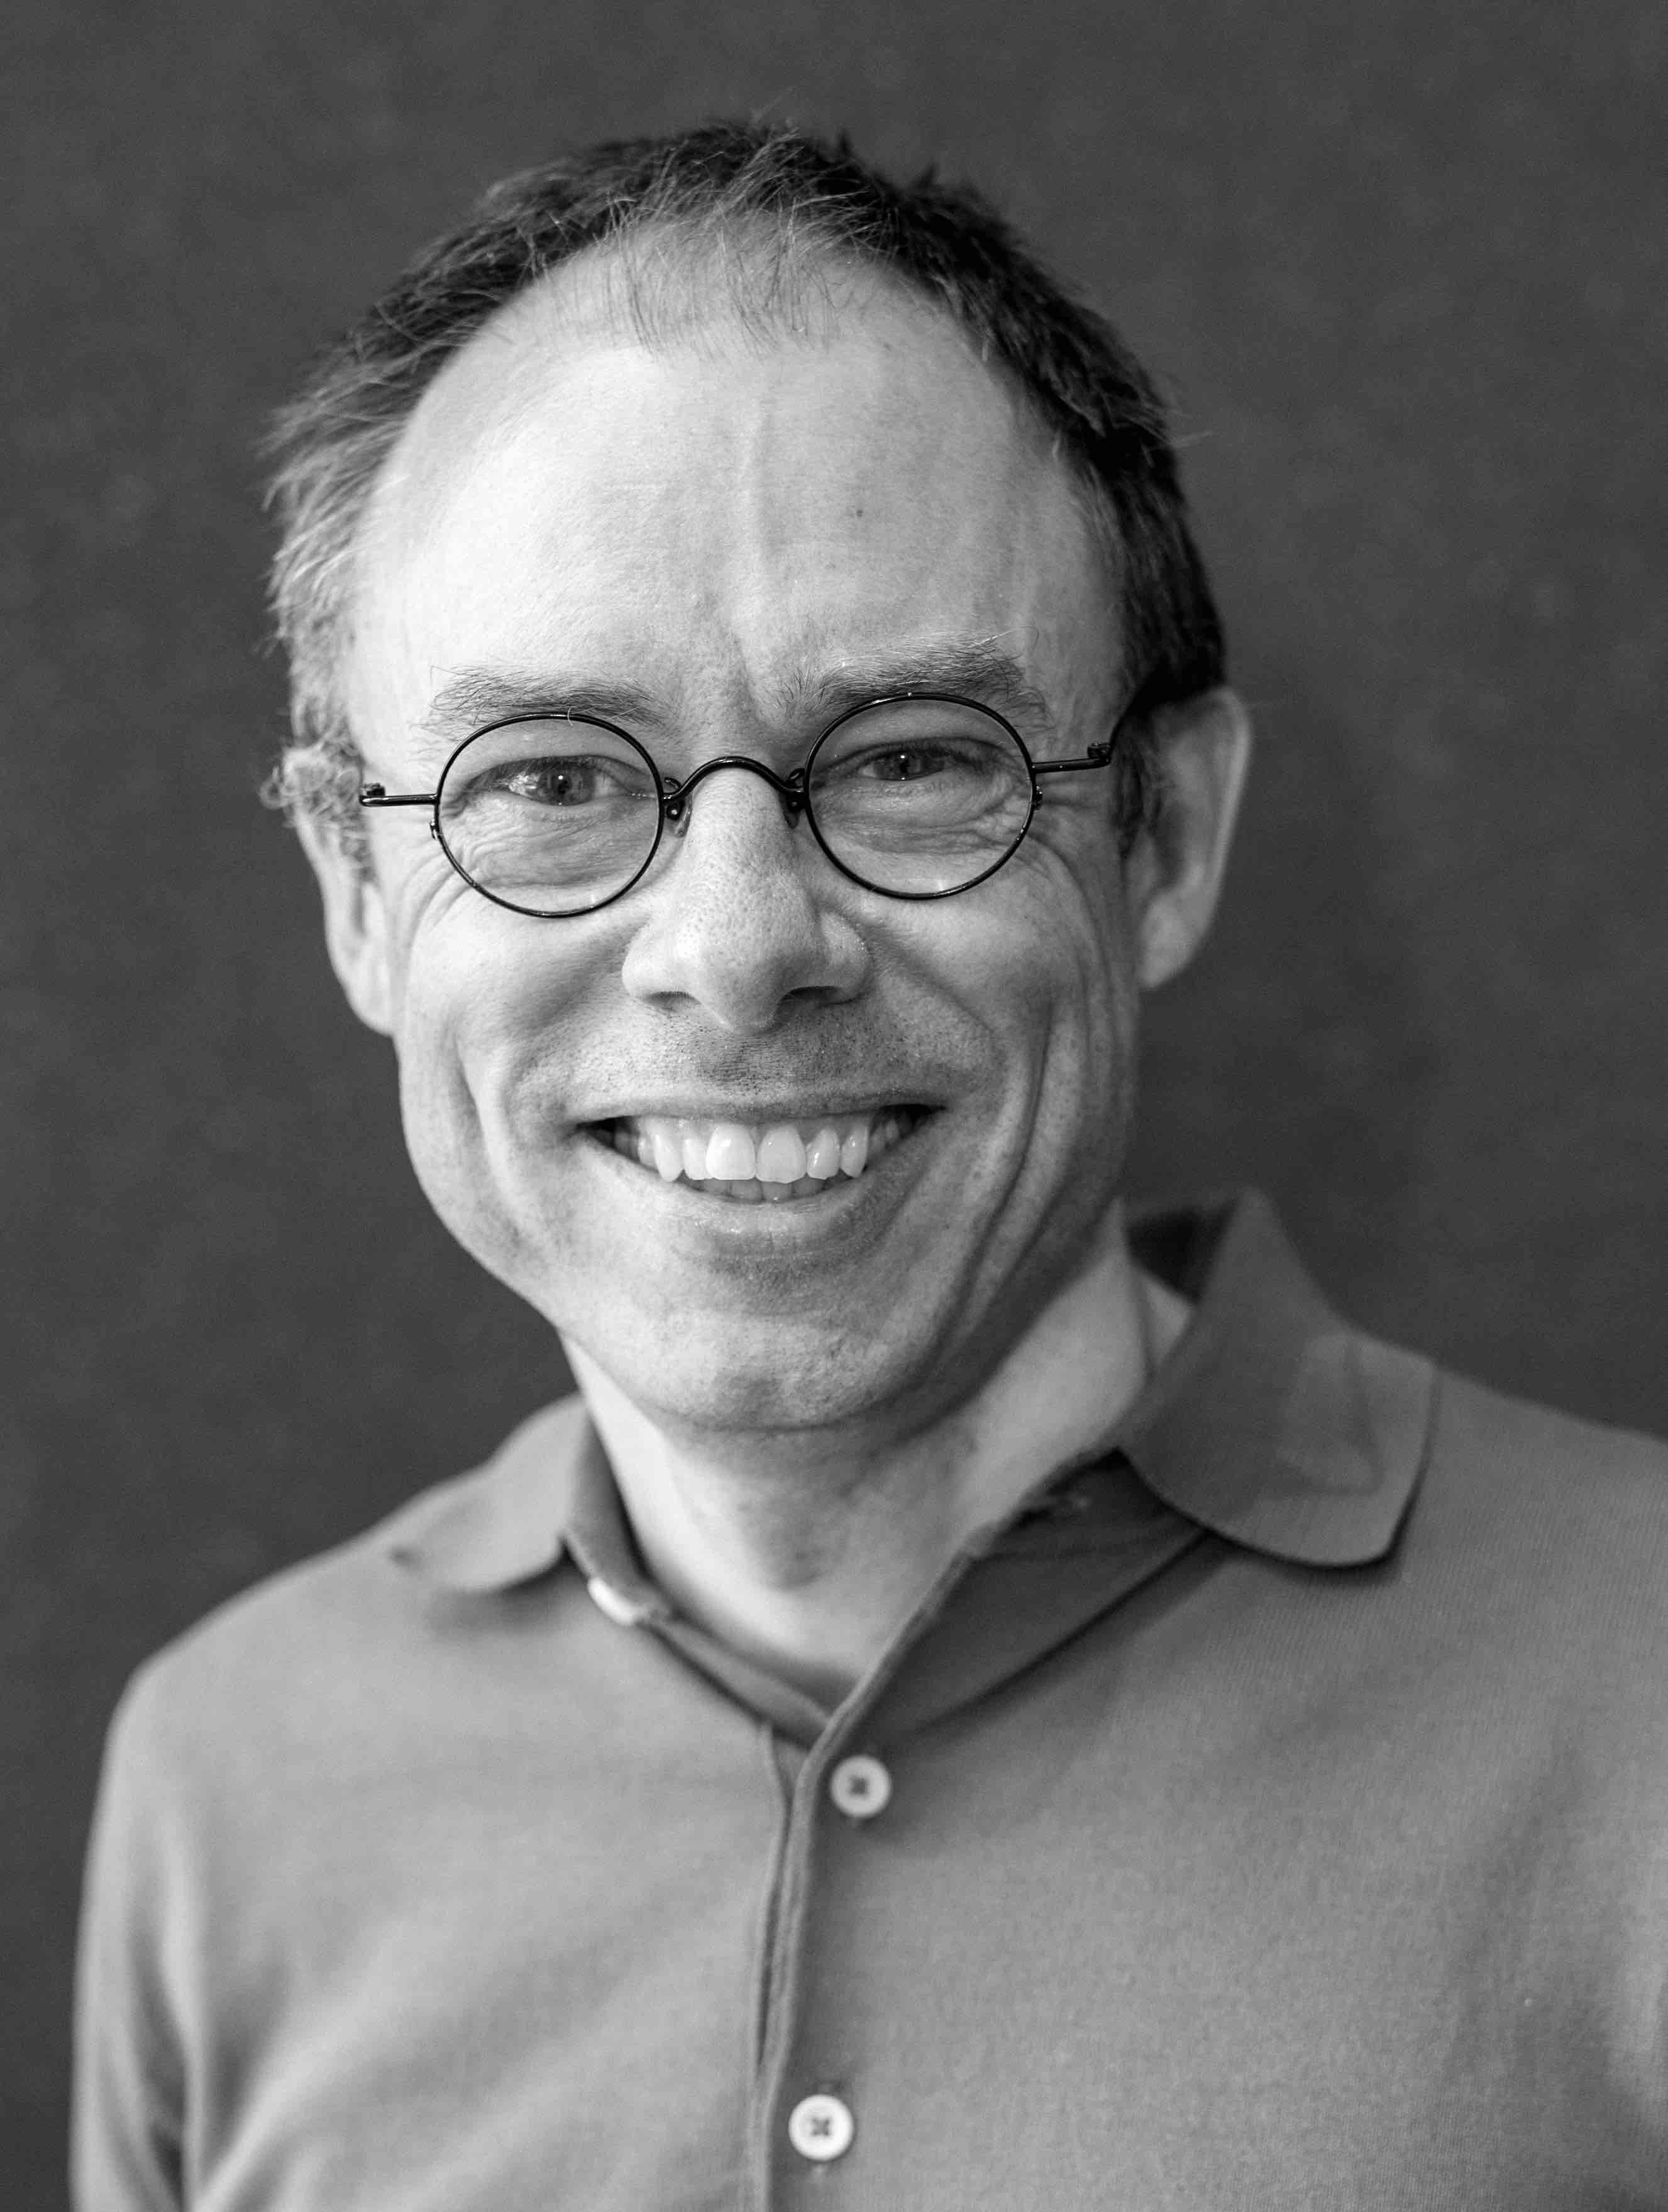
\includegraphics[width=\textwidth]{carsten}
\end{minipage}
\hfill
\begin{minipage}[t][1.5cm][t]{.5\textwidth}
% \hfill
\texttt{
\begin{tabular}{l}
#3 \\
#4 \\[1ex]
\Telefon{ #5}\\
\Letter{ #6}\\
\Mundus{ #7}
\end{tabular}
}
\end{minipage}
}

\newcommand*{\worktitle}[1]{#1}

\newcommand*{\kursus}[2]
{
    \begin{Row}%
      \begin{Cell}{1}
        #1
      \end{Cell}
      \begin{Cell}{3}
        #2
      \end{Cell}
    \end{Row}
}

\newcommand*{\kompetence}[2]
{
    \begin{Row}%
      \begin{Cell}{1}
        #1
      \end{Cell}
      \begin{Cell}{3}
        #2
      \end{Cell}
    \end{Row}
}

\newcommand*{\uddannelse}[3]
{
    \begin{Row}%
      \begin{Cell}{1}
        \worktitle{#1} \\
        #2 % chktex 8
      \end{Cell}
      \begin{Cell}{3}
        #3
      \end{Cell}
    \end{Row}
}

\newcommand*{\job}[5]
{
\begin{Row}%
  \begin{Cell}{1}
    \textbf{#1} \\ [1ex]
    #2 \\
    #3
  \end{Cell}
  \begin{Cell}{3}
    #4 \\ [1ex] #5
  \end{Cell}
\end{Row}
}

